\documentclass[german,masthyd,utf8,lof,lot,hyperref,nomencl]{ihmpub}
\usepackage{setspace}
\author{Max Mustermann}
\title{[Thema]}
\bibfiles{doku}

\birthday{1. Januar 1970}
\placeofbirth{Musterstadt}
\betreuer{Prof. Dr. Niels Schütze}
\matno{1234567}

%-------------Formatierung Symbolverzeichnis-----------
\setlength{\nomlabelwidth}{3cm}
\renewcommand{\nomlabel}[1]{{\bfseries\boldmath#1} \dotfill}
\setlength{\nomitemsep}{-\parsep}

%-------------Hauptteil des Dokuments-----------
\begin{document}
\chapter{Einführung}
\section{Aller Anfang ist schwer}
Gr\"o{\ss}ere Ausarbeitungen an der Professur f\"ur Hydrologie sollen, um ein einheitliches Layout zu erhalten, mittels {\LaTeX} und einer gemeinsamen Formatvorlage erfolgen. 
Dieses Dokument soll den Einstieg in das Erstellen von Dokumenten mit {\LaTeX} erleichtern sowie die Verwendung dieser Formatvorlage erl\"autern.

{\LaTeX} ist eine Dokumentbeschreibungssprache und in dieser Hinsicht HTML nicht un\"ahnlich. 
Es wurde entwickelt um einfach gut aussehende (vor allem wissenschaftliche) Ver\"offentlichungen zu erm\"oglichen. 
F\"ur Grundlagen zu Syntax und Aufbau von {\LaTeX}-Dokumenten sei an dieser Stelle auf zwei hervorragende Einf\"uhrungen, und gleichzeitig Referenzen, verwiesen: \citet{kochbuch} sowie \cite{rudl}. 
Weiterhin ist zu {\LaTeX} auch einschl\"agige Literatur vorhanden -- genannt werden sollen an dieser Stelle exemplarisch \cite{begleiter} und \cite{kopka}. 
Im Folgenden soll im Besonderen auf den Umgang mit der hier zur Verf\"ugung gestellten Formatvorlage eingegangen werden.




\section{Einführung}
Die Schlüsselelemente von Entscheidungsprozessen in der Bewirtschaftung
von Hydrosystemen\footnote{synonym wird oft auch der Begriff ``Wasserressourcenmanagement''
gebraucht} sind Ziele (siehe auch Abb~\ref{fig:bild1}),
Planungsszenarien und Bewirtschaftungsregeln sowie Entscheidungsträger
und andere Akteure, die in den Entscheidungsprozessen involviert sind sowie die betrachteten Hydrosysteme in
Form von mathematischen Beschreibungen (mathematische Modelle). Gewöhnlich
sind alle Elemente komplex strukturiert.

%%%%%%%%%%%%%%%%%%%%%%%%%%%%%%%%%%%%%%%%%%%%%%%%%%%%%%%%%%%%%%%
\begin{figure}[tbp]
  \begin{center}
    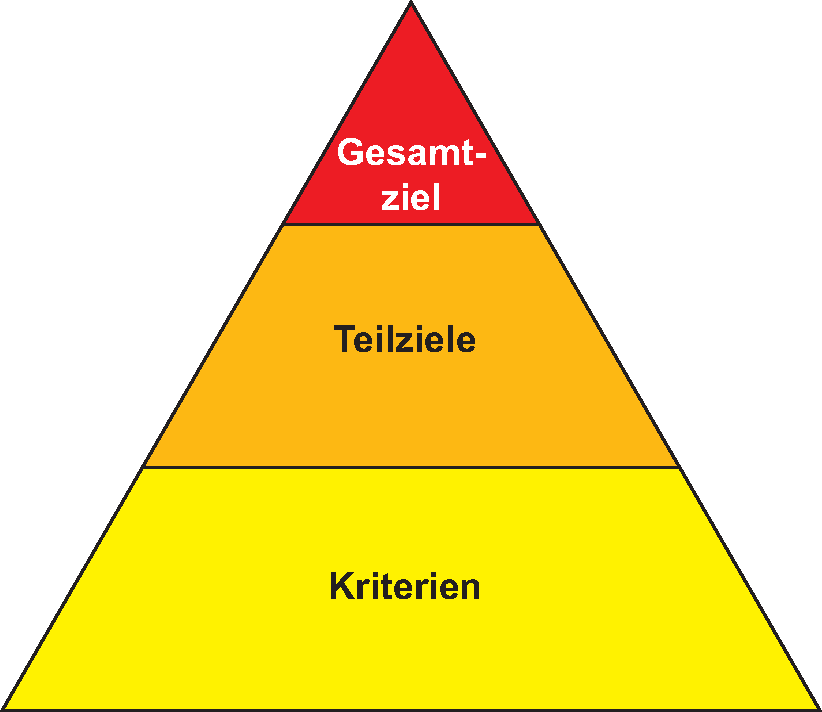
\includegraphics[width=0.45\textwidth]{Bild1a.pdf} 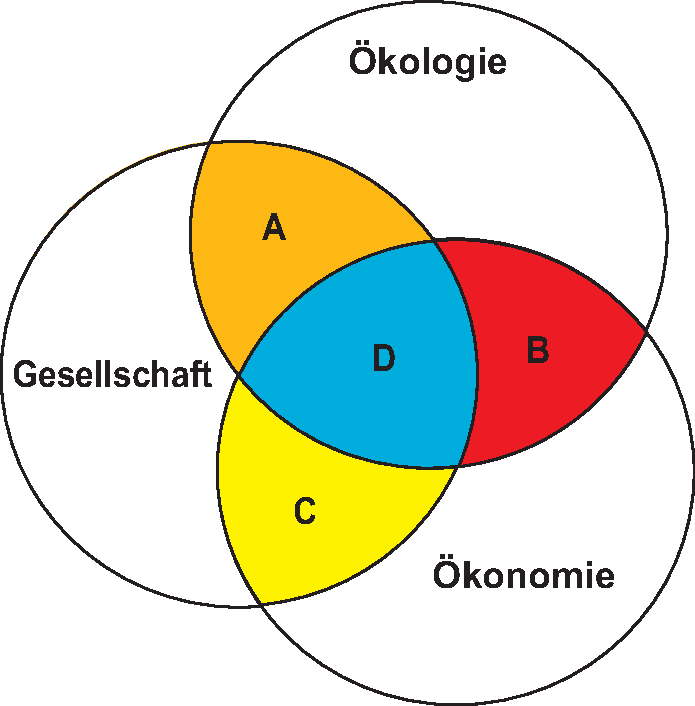
\includegraphics[width=0.45\textwidth]{Bild1b.pdf}
    \caption{Entscheidungsziele in der integrierten Bewirtschaftung von Hydrosystemen}
    \label{fig:bild1}
  \end{center}
\end{figure}

\section{Infiltrationsmodelle}

Die in Tabelle~\ref{tab:tab1} beschriebenen Infiltrationsmodelle
und in Tabelle sind empirische Modelle, bei denen der Systemzustand
keine Rolle spielt. Daher kann die kummulative Infiltration sofort
für alle Zeitpunkte $t$ berechnet werden:

\begin{equation}
I=\boldsymbol{f}(t).
\end{equation}
\nomenclature[t]{$t$}{Zeit}
\nomenclature[f]{$f$}{Funktion}
\nomenclature[I]{$I$}{kummulative Infiltration}
\nomenclature[Q]{$\bar{Q}$}{mittlerer Durchfluss}
\begin{table}[h!]
\caption{Infiltrationsmodelle.}\label{tab:tab1}
\begin{centering}
\begin{tabular}{|c|c|}
\hline 
Philip Modell & Kostiakov Modell\tabularnewline
\hline 
Swartzendruper Modell & modified Kostiakov Modell\tabularnewline
\hline 
Horton Modell & revise modified Kostiakov Modell\tabularnewline
\hline 
SCS Modell & \tabularnewline
\hline 
\end{tabular}
\par\end{centering}
\end{table}

%%%%%%%%%%%%%%%%%%%%%%%%%%%%%%%%%%%%%%%%%%%%%%%%%%%%%%%%%%%%%%%%%%%

\end{document}
